\begin{figure}[H]
	\centering 
	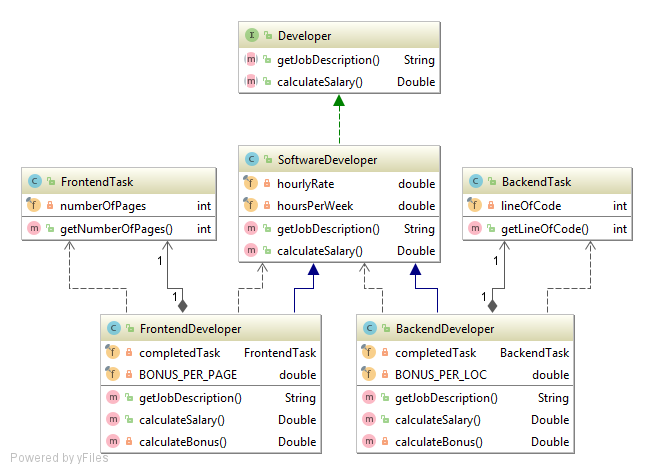
\includegraphics[clip, trim=0cm 0cm 0cm 0cm, scale=0.8]{../uml/q6_ClassDiagram.png}
	\caption{Functional Inheritance Diagram}
\end{figure}

\begin{itemize}
\item In this example, we have a functional inheritance. SoftwareDeveloper class implemented Developer interface, which has two methods, including getJobDescription() and calculateSalary(). The class has a default implementation for all software developers. BackendDeveloper and FrontendDeveloper classes inherited from SoftwareDeveloper class and redefined its methods. These child classes overrode inherited methods and implemented their functionalities.
\item One can find implementation code and unit tests in our submission under "Q6" package.
\end{itemize}